% Created 2011-08-25 Thu 15:03
\documentclass[11pt]{article}
\usepackage[utf8]{inputenc}
\usepackage[T1]{fontenc}
\usepackage{graphicx}
\usepackage{longtable}
\usepackage{float}
\usepackage{wrapfig}
\usepackage{soul}
\usepackage{amssymb}
\usepackage{hyperref}


\title{Documentation of MooseGUI}
\author{}
\date{25 August 2011}

\begin{document}

\maketitle

\setcounter{tocdepth}{3}
\tableofcontents
\vspace*{1cm}
\section{Getting Started}
\label{sec-1}


  The script to start the GUI for MOOSE is moosegui.py. Depending on where it is installed, you can enter the following in a command prompt:
  >python \{full path of moosegui.py\}

  If you install it from a binary package, it should already be in your path and have execute permission set. In that case just entering
  >moosegui.py
  should fire up the GUI.

  If you are running it for the first time, a graphical wizard will appear to confirm some details. It has three pages. Verify if the details in these pages are correct. Other wise select the appropriate values. The initial page contains general information about MOOSE and the wizard itself.

  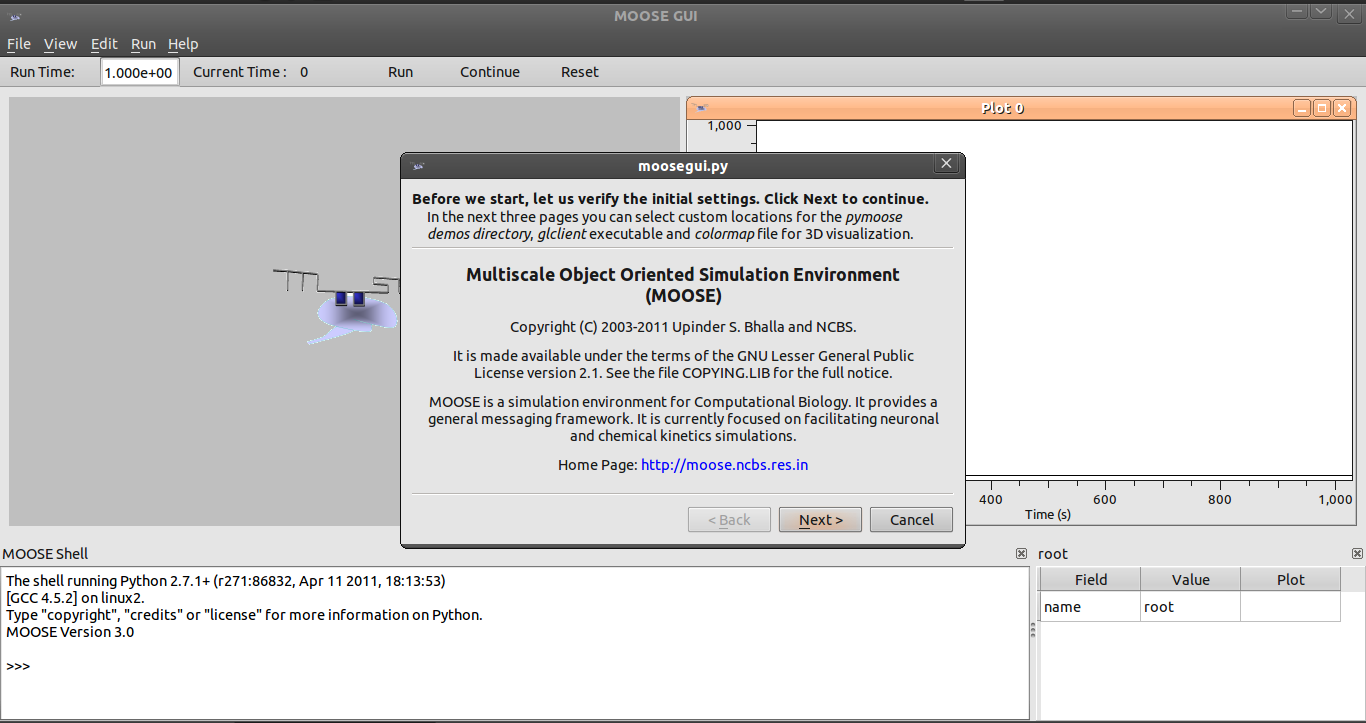
\includegraphics[width=14cm]{/home/chaitu/Desktop/moose/pymoose/gui/qt/documentation/firsttime1.png}

  Click next and you will be prompted to select the directory containing the PyMOOSE demos. On Linux systems, these are installed in usr/share/doc/moose1.3/DEMOS/pymoose. Verify that the contents of the text box labeled ``PyMOOSE demos directory'' has the correct location of the PyMOOSE demos. Otherwise, click the Browse button next to it and browse to the appropriate directory and click Open button on the pop-up dialog.

  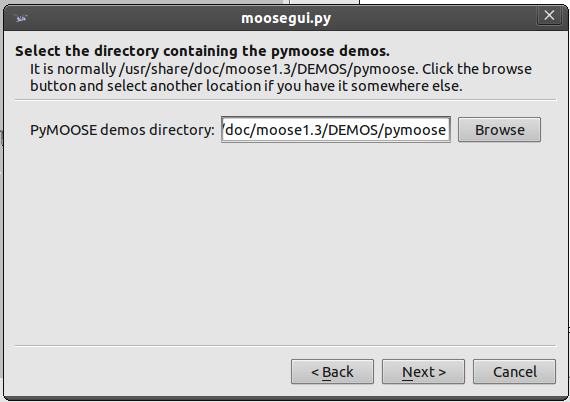
\includegraphics[width=8cm]{/home/chaitu/Desktop/moose/pymoose/gui/qt/documentation/firsttime2.png}

  After clicking next you will reach the final page in the wizard. Here you specify a colormap file for OpenGL-based 3D visualization. Select any of the files in the colormaps directory and click Finish.

  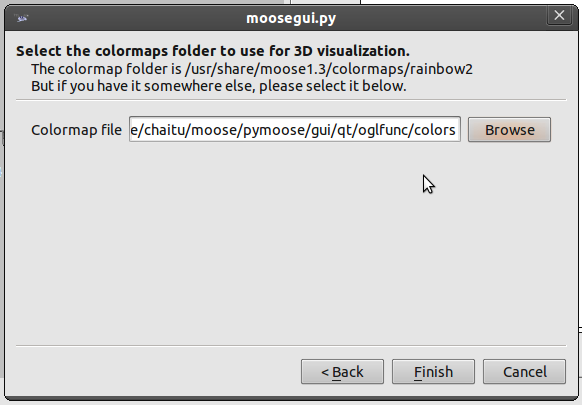
\includegraphics[width=8cm]{/home/chaitu/Desktop/moose/pymoose/gui/qt/documentation/firsttime4.png}


\section{MooseGUI layout}
\label{sec-2}


  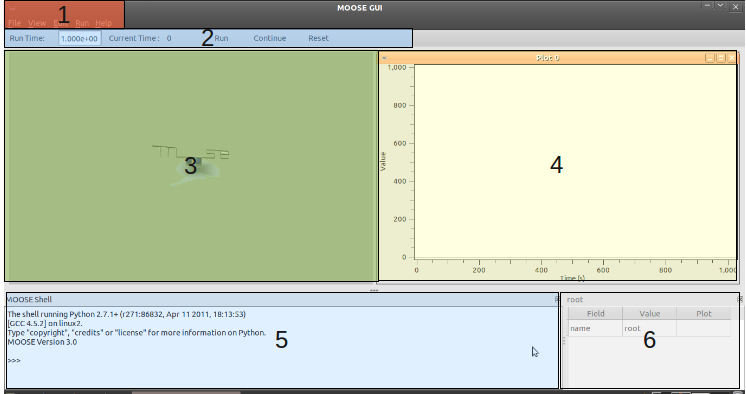
\includegraphics[width=14cm]{/home/chaitu/Desktop/moose/pymoose/gui/qt/documentation/layout.png}
  
\begin{enumerate}
\item Menu
\item Simulation Toolbar
\item Visualization Area
\item Plotting Area
\item Moose Shell
\item Object Editor
\item Simulation Control Panel*
\item Moose Element Tree*
\item Moose Classes Panel*
\end{enumerate}
  
  *by default not shown at startup, to make them visible: In \hyperref[sec-2]{Menu}>View> and check on corresponding item to show  


\section{Load Models}
\label{sec-3}


  In the menu area, click on \hyperref[sec-2]{Menu}>File>Load Model (or alternatively Ctrl+L)

  A dialog box as shown would show up. Nagivate to the model and open.

  Currenly only one model can be loaded in one session.
  
  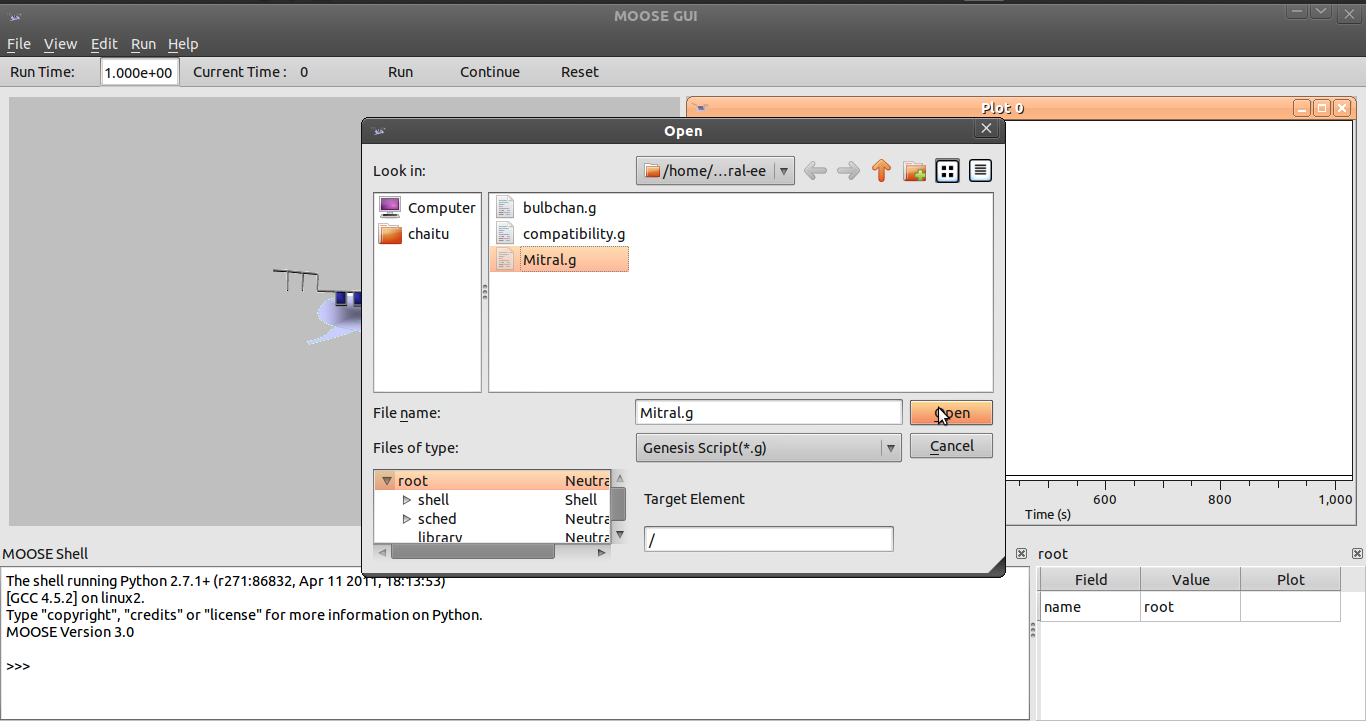
\includegraphics[width = 14cm]{/home/chaitu/Desktop/moose/pymoose/gui/qt/documentation/loadmodel.png}

\subsection{Kinetikit Models}
\label{sec-3.1}

   In addition to regular GENESIS scripts, the GUI recognizes .g files that contain kinetikit models. Kinetikit models have the commands to plot variables of interest. When one load the model, all these plots are added to the available plot window in \hyperref[sec-2]{Plotting Area}. Moreover,  A graphical representation of the reaction network is displayed in the \hyperref[sec-2]{Visualization Area} and the plots in the \hyperref[sec-2]{Plotting Area}. 
   
   For example, load Kholodenko.g from DEMOS/kholodenko directory to get the following:

  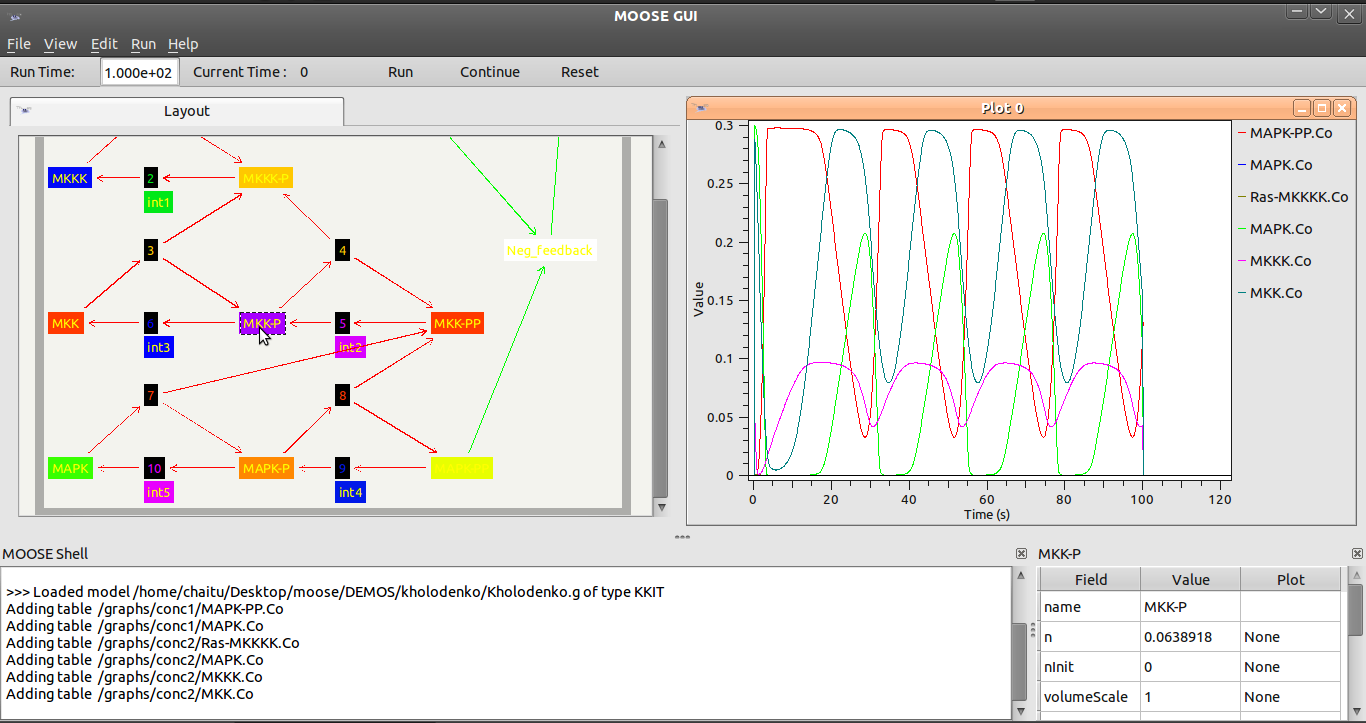
\includegraphics[width = 14cm]{/home/chaitu/Desktop/moose/pymoose/gui/qt/documentation/kinetikit.png}

   One can double click any item in the \hyperref[sec-2]{Visualizaton Area} and it  will be opened in the \hyperref[sec-2]{Object Editor} for the underlying MOOSE object. One can modify the properties of the objects (for example the initial concentration of a substrate) in the \hyperref[sec-2]{Object Editor}. (In the above example `MKK-P' has been double clicked)

   
\subsection{Neural Models}
\label{sec-3.2}

    In the visualization area the cell is displayed. By default only if single celled models are visualized. (To change this see, \hyperref[sec-3.2]{New GL Windows})
    
    For example, load mitral.g from DEMOS/mitral-ee directory to get the following:  (currently .py and .g models are supported) 

  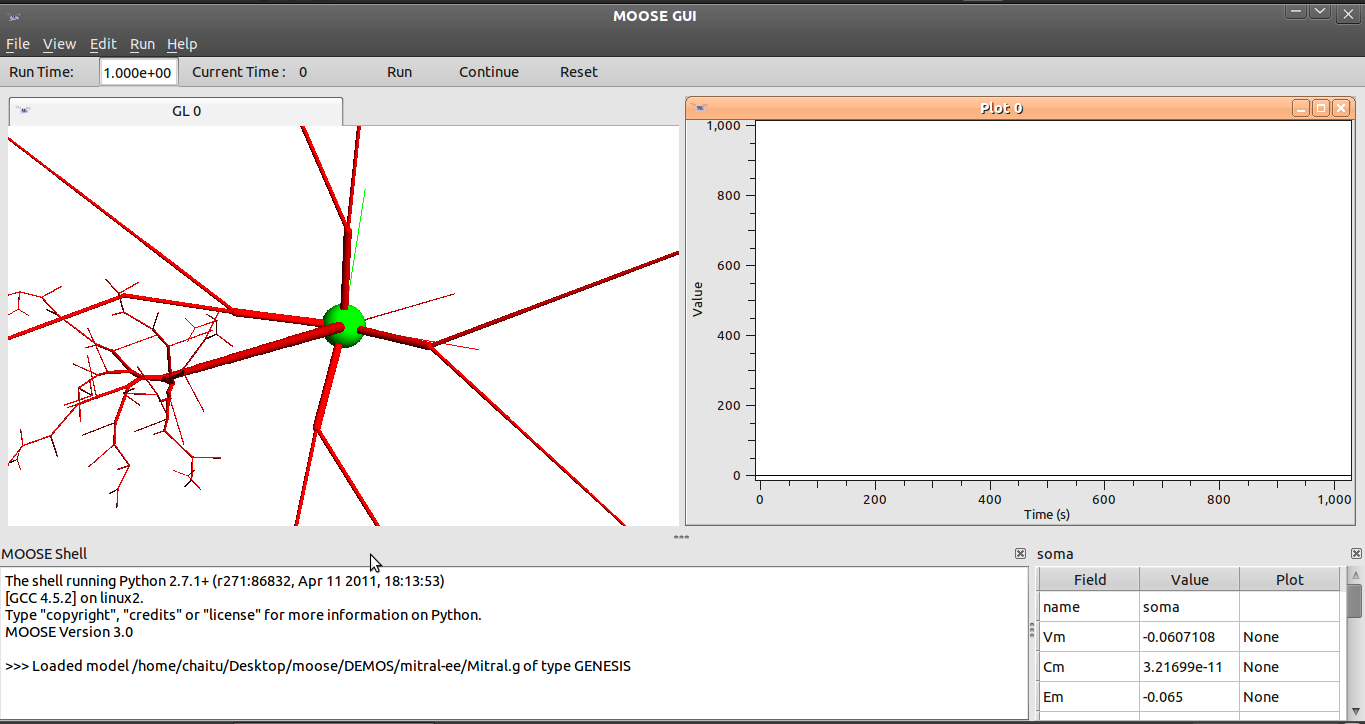
\includegraphics[width = 14cm]{/home/chaitu/Desktop/moose/pymoose/gui/qt/documentation/clickedSoma.png}
    
\begin{itemize}
\item Interaction: 
      Click on a compartment to open the the compartment properties in the \hyperref[sec-2]{Object Editor}. Selected compartment is highlighted in green color. (In the above example `soma' has been clicked. Notice the updation of the object editor fields)
\item Navigation:
      One can navigate in this area using mouse and keyboard.

\begin{itemize}
\item Click and drag to rotate model.
\item Use arrow keys to pan the model.
\item Mouse wheel to zoom.
\end{itemize}

\end{itemize}
    
\begin{itemize}
\item New GL Windows:
      To add new GL Windows or to display models with more than one cell \hyperref[sec-2]{Menu}>View>New GL Window  A Dialog would then appear, here add the cells to be visualized. Also one can select the style in which, the visualization be displayed. The field you wish to visualize, while specifying the range of the values of the field and the choice of colormap.
\end{itemize}
  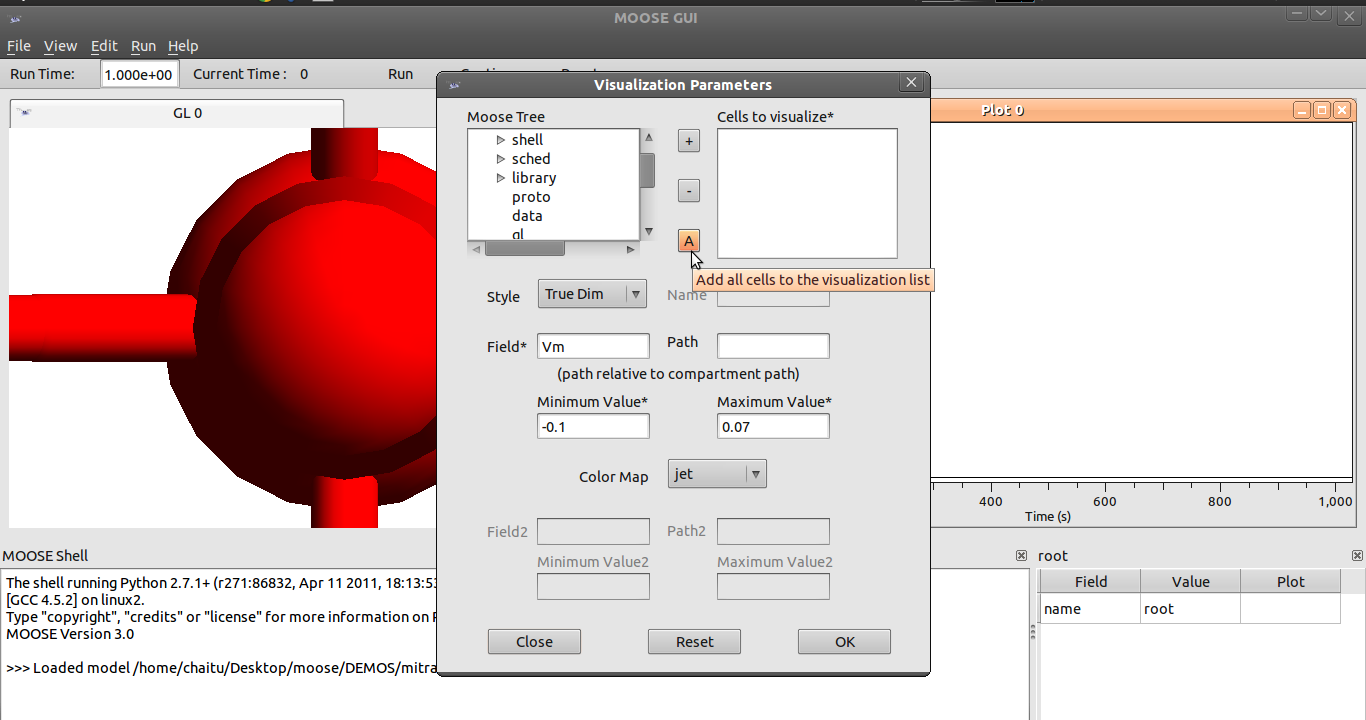
\includegraphics[width = 14cm]{/home/chaitu/Desktop/moose/pymoose/gui/qt/documentation/newGL.png}

      
\section{Record field values and Plots}
\label{sec-4}

  
  To record field values of a particular moose object, it must be added via the \hyperref[sec-2]{Object Editor}. 
\begin{itemize}
\item The corresponding field of interest is to be dragged onto the plot window in \hyperref[sec-2]{Plotting Area} (OR)
\item Click the third column in the \hyperref[sec-2]{Object Editor}, to bring up a combo box from which the plot window name (`Plot 0' as shown below) can be selected
\end{itemize}
  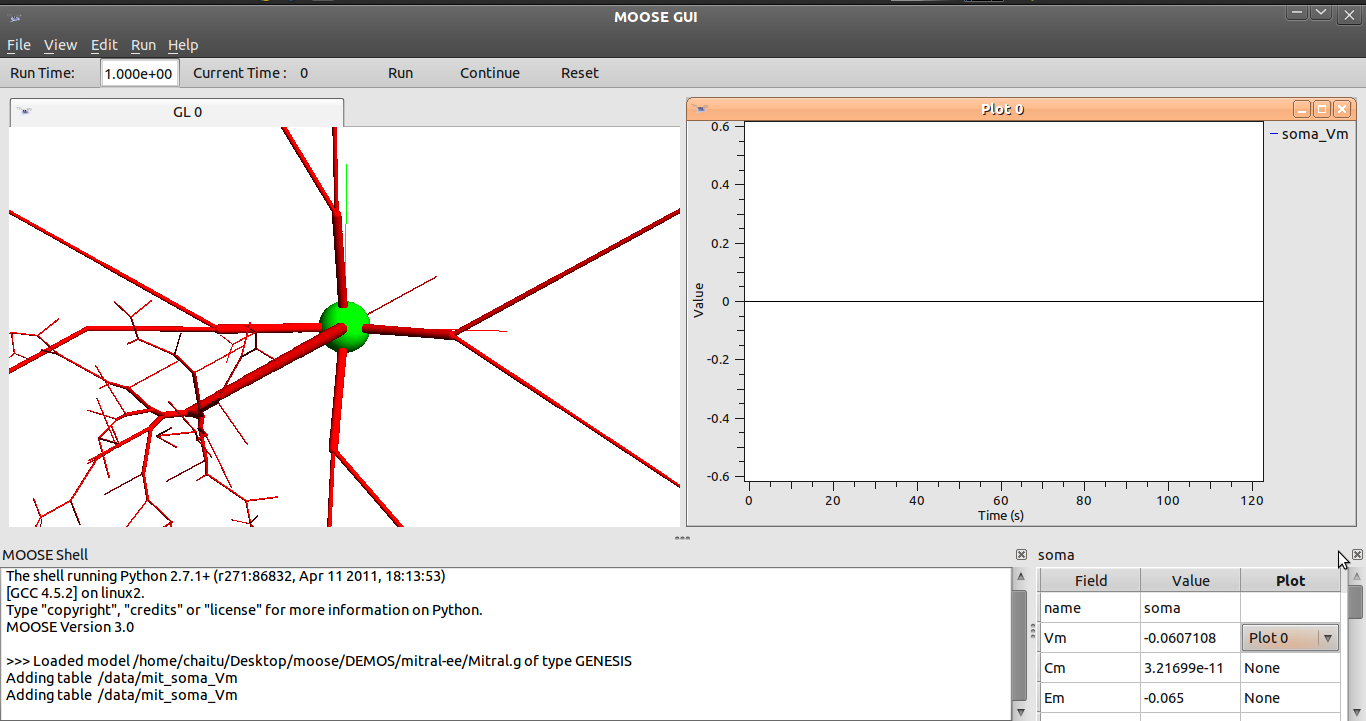
\includegraphics[width=14cm]{/home/chaitu/Desktop/moose/pymoose/gui/qt/documentation/plotCombo.png}
 
  One can add new plot windows to the \hyperref[sec-1]{Plotting Area} (in \hyperref[sec-2]{Menu}>View>New Plot Window), by default 1 plot is shown (named Plot 0). 
  To close the plots, right click on the window pane of the corresponding plot window. 
  Change the layout of the plots by changing it from \hyperref[sec-2]{Menu}>View> Tabbed View / Cascading Plots

\section{Run Simulation}
\label{sec-5}

  
  To run the simulation, use the \hyperref[sec-2]{Simulation Toolbar} Use the `Run','Continue' and `Reset' buttons here for the corresponding actions.
  
  Further, to change the time step interval of the simulation and the plot/visualization update interval use the simulation control (by default not visible, to make visible, check \hyperref[sec-2]{Menu}>View>Simulation Control)

\section{Save}
\label{sec-6}


  To save plots use \hyperref[sec-2]{Menu}>File>Save Plots (Ctrl+S). Saving action prompts user for the directory in which one wishes to save the files, this dumps all the data on the plot windows into corresponding fieldname.plot files. (One can save plots only after running the simulation)

\section{Reset Settings}
\label{sec-7}


  To reset the layout of the GUI (also resets the `First Time Wizard') use \hyperref[sec-2]{Menu}>File>Reset Settings, the settings are restored only after restarting moosegui.py

\end{document}
